\section{Design}
\label{sec:desgin}
\lhead{\thesection \space Design}
This chapter deals with the design artefacts that were created during this project. First the functionality of the \textit{Connected.Football} application will be explained using a State Machine Diagram and an Activity Diagram. The second chapter deals with the visual design of the application. After that a brief definition of the \textit{Vote4Fun} object is given. Finally the design of the components that were designed during this projects are explained. 

\subsection{Functionality}
\label{ssec:functionality}

Since the application is supposed to offer a certain set of features to the user, it needed to be defined what kind of functionality was necessary to ensure that a user could interact with all the features the application has to offer. This section details this set of features and their functionality.
\newline
Each functionality is described using a set of diagrams, such as state machine or activity diagrams. A visual representation can also be found in \textit{\ref{ssec:visual_design} \nameref{ssec:visual_design}}.

\subsubsection{Creating a new Poll}
\label{sssec:creating_a_new_poll}

Since the \textit{Vote4Fun} extension is about creating a poll and letting users vote on it, the actual creation of such a poll is of course an important and arguably biggest piece of functionality. The polls are divided into two categories, which are a regular and an "on-the-fly" poll.
\newline
The regular poll is created for one specific team, as shown in Figure \ref{fig:state_machine_diagram_create_poll}. The owner of the poll simply picks a team and is able to add guests to the poll afterwards. Each guest is checked for validity, in this case whether the entered email address representing the guest is an active user of \textit{Connected.Football}. This can be repeated for multiple users. An "on-the-fly" poll does not require a team, but rather a set of email addresses, which do not need to be registered on \textit{Connected.Football}. Once the owner has entered the email addresses, a temporary team is created (see \textit{\ref{sssec:creating_temp_team} \nameref{sssec:creating_temp_team}}).
\newline
In both cases, the poll has a set of users. Once the owner enters information regarding the deadline and exercises to be voted upon, the poll itself is created. This is followed by notifications being sent to all users participating in the poll.

\begin{figure}[H]
    \begin{center}
        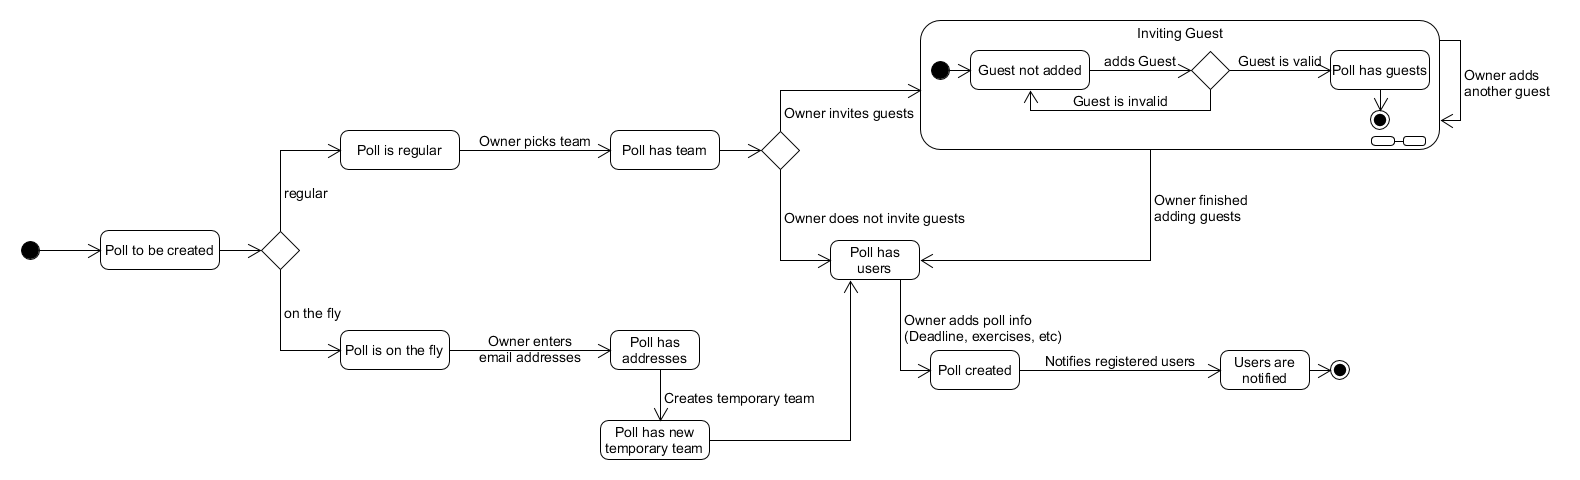
\includegraphics[width=1\textwidth]{images/diagrams/state_machine_diagrams/StateDiagram_CreatePoll.png}
        \caption{State Machine Diagram Create Poll}
        \label{fig:state_machine_diagram_create_poll}
    \end{center}
\end{figure}

Figure \ref{fig:activity_diagram_create_poll} shows the activity diagram that describes the process of creating a new exercise poll. 
\newline
The process starts when the actor selects "\textit{Create New Exercise Poll}" while creating or editing a training. After that the application will guide the actor through the process of creating a new poll. First the actor enters a title for the poll. Then the system lists all available exercises from the \textit{Connected.Football} environment and the actor can select up to 4 but at least 2 exercises that the player later on can vote for. After selecting the exercises the actor is prompted to enter a deadline for the poll. The system will then check if the deadline is in the future and will deny dates that are in the past. Finally the actor has some options e.g. if the players are able to see intermediate results, if the players can see the final results and notification type. The system will then store the poll in the \textit{Connected.Football} environment and send the notifications to the players. 


\begin{figure}[H] 
    \begin{center}
        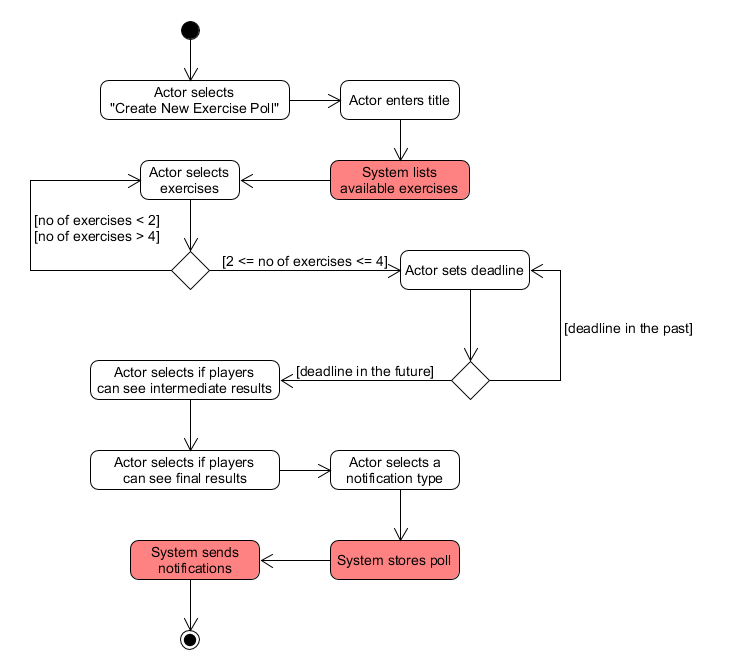
\includegraphics[width=0.8\textwidth]{images/diagrams/activity_diagrams/ActivityDiagram_CreateExercisePoll.png}
        \caption{Activity Diagram Create Poll}
        \label{fig:activity_diagram_create_poll}
    \end{center}
\end{figure}

\subsubsection{Creating a Temporary Team}
\label{sssec:creating_temp_team}

As mentioned in \textit{\ref{sssec:creating_a_new_poll} \nameref{sssec:creating_a_new_poll}}, when an "on-the-fly" poll is created, a new temporary team is created as well. This team consists of people that may or may not be registered with the \textit{Connected.Football} platform. Unfortunately, this functionality was not implemented in time, but since it is required for Epic 3 (see \textit{\ref{sssec:epic3} \nameref{sssec:epic3}}, it is mentioned for the sake of completeness and for future reference.
\newline
As seen in Figure \ref{fig:state_machine_diagram_create_temp_team}, the process starts with the owner of the poll entering an email address representing the person they want to add to the temporary team. If the email is not properly formatted, the entry is discarded. If the format is correct, the address is stored and the owner can either add another email address or they can continue.
\newline
The \textit{Connected.Football} platform than checks for every entered email address whether a user with the same address is already registered. If that is the case, the reference to the already existing user is stored in the temporary team and the user is sent a push notification. If not, the platform creates a callback and sends an invitation to the email address. This invitation was supposed to be handled by \textit{Firebase}, which provides functionality for such an on-boarding process. If the user follows this invitation, the callback is triggered, which stores the new user in the temporary team, once they have completed their registration.

\begin{figure}[H]
    \begin{center}
        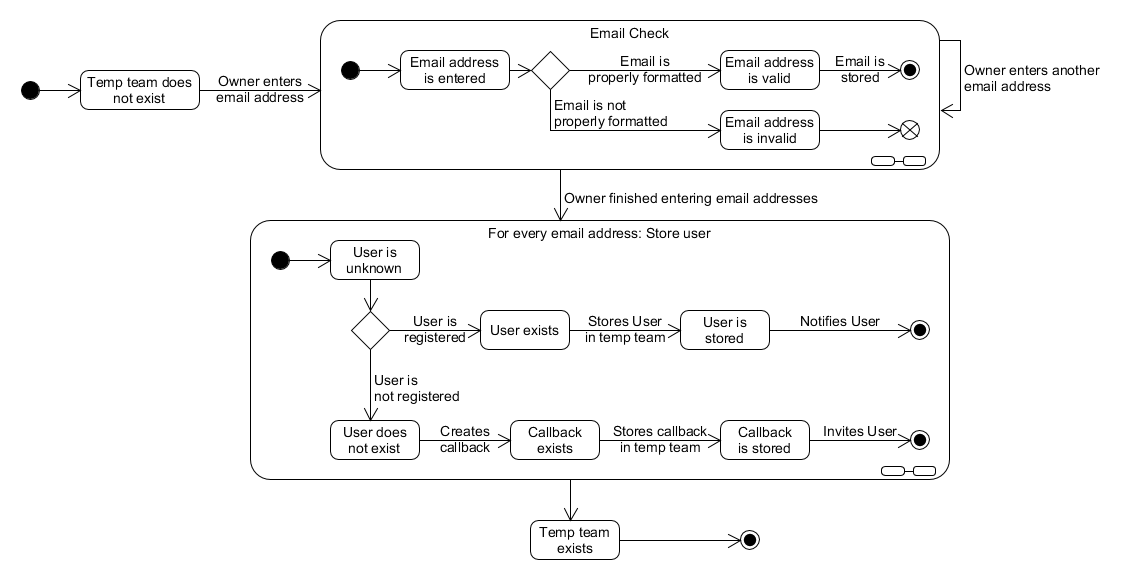
\includegraphics[width=1\textwidth]{images/diagrams/state_machine_diagrams/StateDiagram_CreateTempTeam.png}
        \caption{State Machine Diagram Create Temporary Team}
        \label{fig:state_machine_diagram_create_temp_team}
    \end{center}
\end{figure}

\subsubsection{Voting on an Exercise Poll}
\label{sssec:voting_on_exercise_poll}
The following activity diagram (Figure \ref{fig:activity_diagram_vote_on_poll}) shows how the process of voting on a poll works. First the actor opens an exercise poll in the \textit{Connected.Football} application where the system will list all exercises that can be voted for. The next step for the actor then is to select an exercise that he wants to vote for. After the actor selected an exercise the system shows a confirmation dialog to confirm that the actor wants the particular exercise. If he changed his mind and wants to vote for another exercise he can deny the confirmation dialog. When the actor selects confirm the system will store the vote in the \textit{Connected.Football} environment. 

\begin{figure}[H]
    \begin{center}
        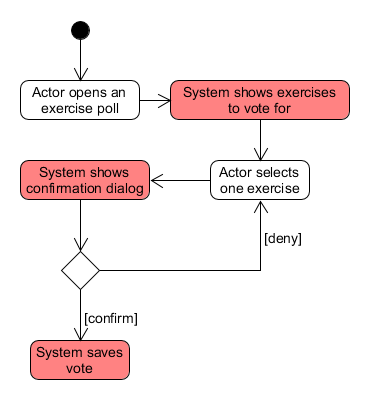
\includegraphics[width=0.5\textwidth]{images/diagrams/activity_diagrams/ActivityDiagram_VoteOnExercisePoll.png}
        \caption{Activity Diagram Vote on Poll}
        \label{fig:activity_diagram_vote_on_poll}
    \end{center}
\end{figure}

\subsubsection{Entering a Promotion Code}
\label{sssec:entering_promotion_code}
The activity diagram "Enter Promotion Code" shows the process of entering a promotion code to activate a trial period for a feature. To start this process the actor has to navigate to his or her account settings. In the account settings the actor will see an item labelled "Enter Promotion Code". This item has to be selected and the actor is prompted to enter a promotion code. After the actor entered a promotion code the system will check if the code was correct. If the code was incorrect the system will show a negative confirmation and the actor will redirected to enter the promotion code again. When the code was correct then the system will show a positive confirmation and it will start the trial period for the actor.

\begin{figure}[H]
    \begin{center}
        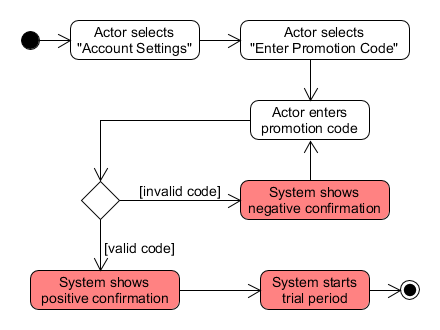
\includegraphics[width=0.6\textwidth]{images/diagrams/activity_diagrams/ActivityDiagram_EnterPromotionCode.png}
        \caption{Activity Diagram Enter Promotion Code}
        \label{fig:activity_diagram_enter_promotion_code}
    \end{center}
\end{figure}

\subsection{Visual Design}
\label{ssec:visual_design}

For expressing our ideas of the visual design of the features to be implemented mock-ups are used. In order to create them different tools like \textit{Umlet}, \textit{Gimp}, \textit{Pencil}, ... were utilised.
\newline
Figure \ref{fig:mockup_main} shows the mockup for creating a new poll. To create a new poll a title, a deadline, a team and exercises have to entered. It is also possible to make the results available during the poll via a selected check box. The coach can also set a flag that the players will be notified if the poll is close to finish.  
\begin{figure}[H]
    \begin{center}
        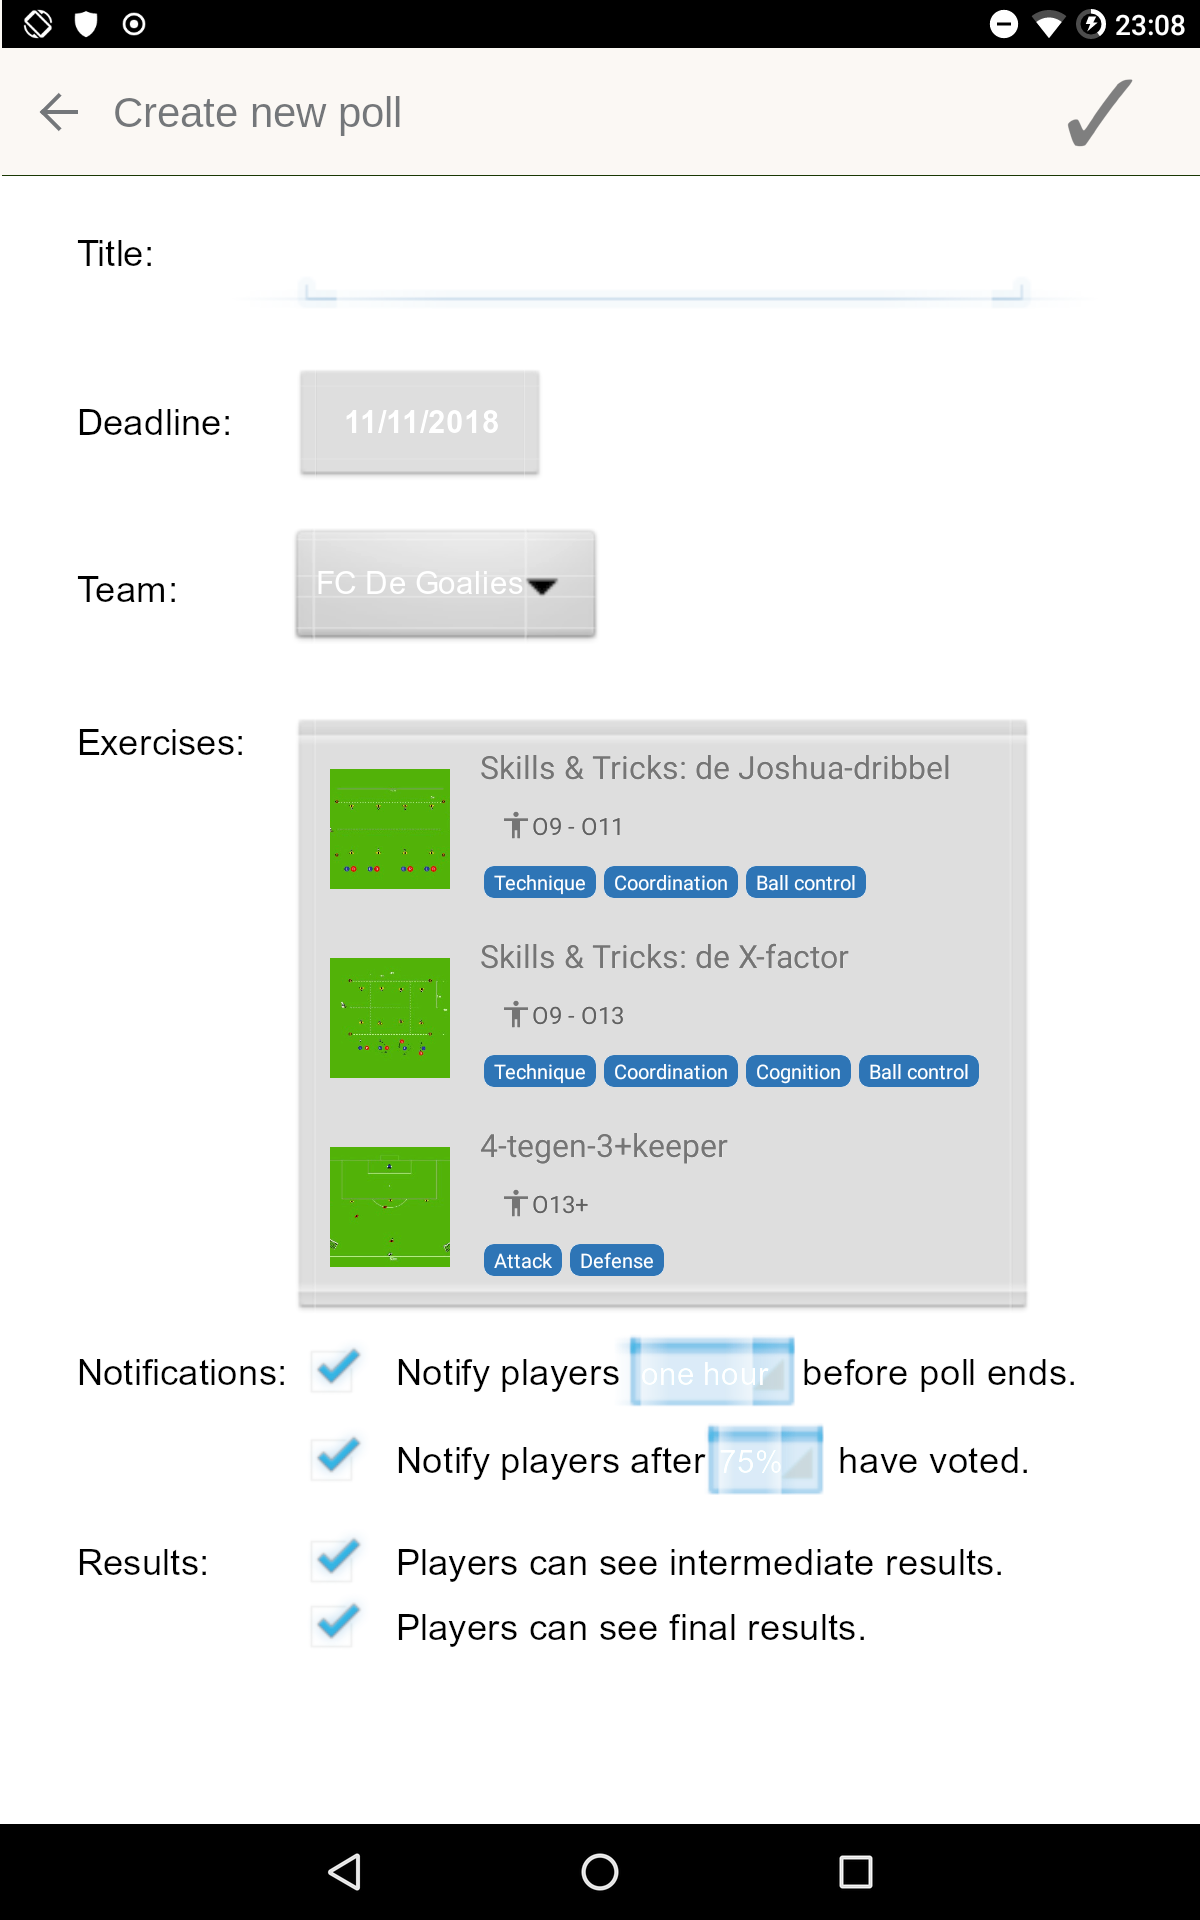
\includegraphics[width=0.4\textwidth]{images/mockups/create.png}
        \caption{Mockup Create Dialog}
        \label{fig:mockup_create}
    \end{center}
\end{figure}

The mockup in Figure \ref{fig:mockup_main} shows the overview of the polls. This overview shows the coach which polls for his are currently running or have finished. He is also able to delete a poll. 
\begin{figure}[H]
    \begin{center}
        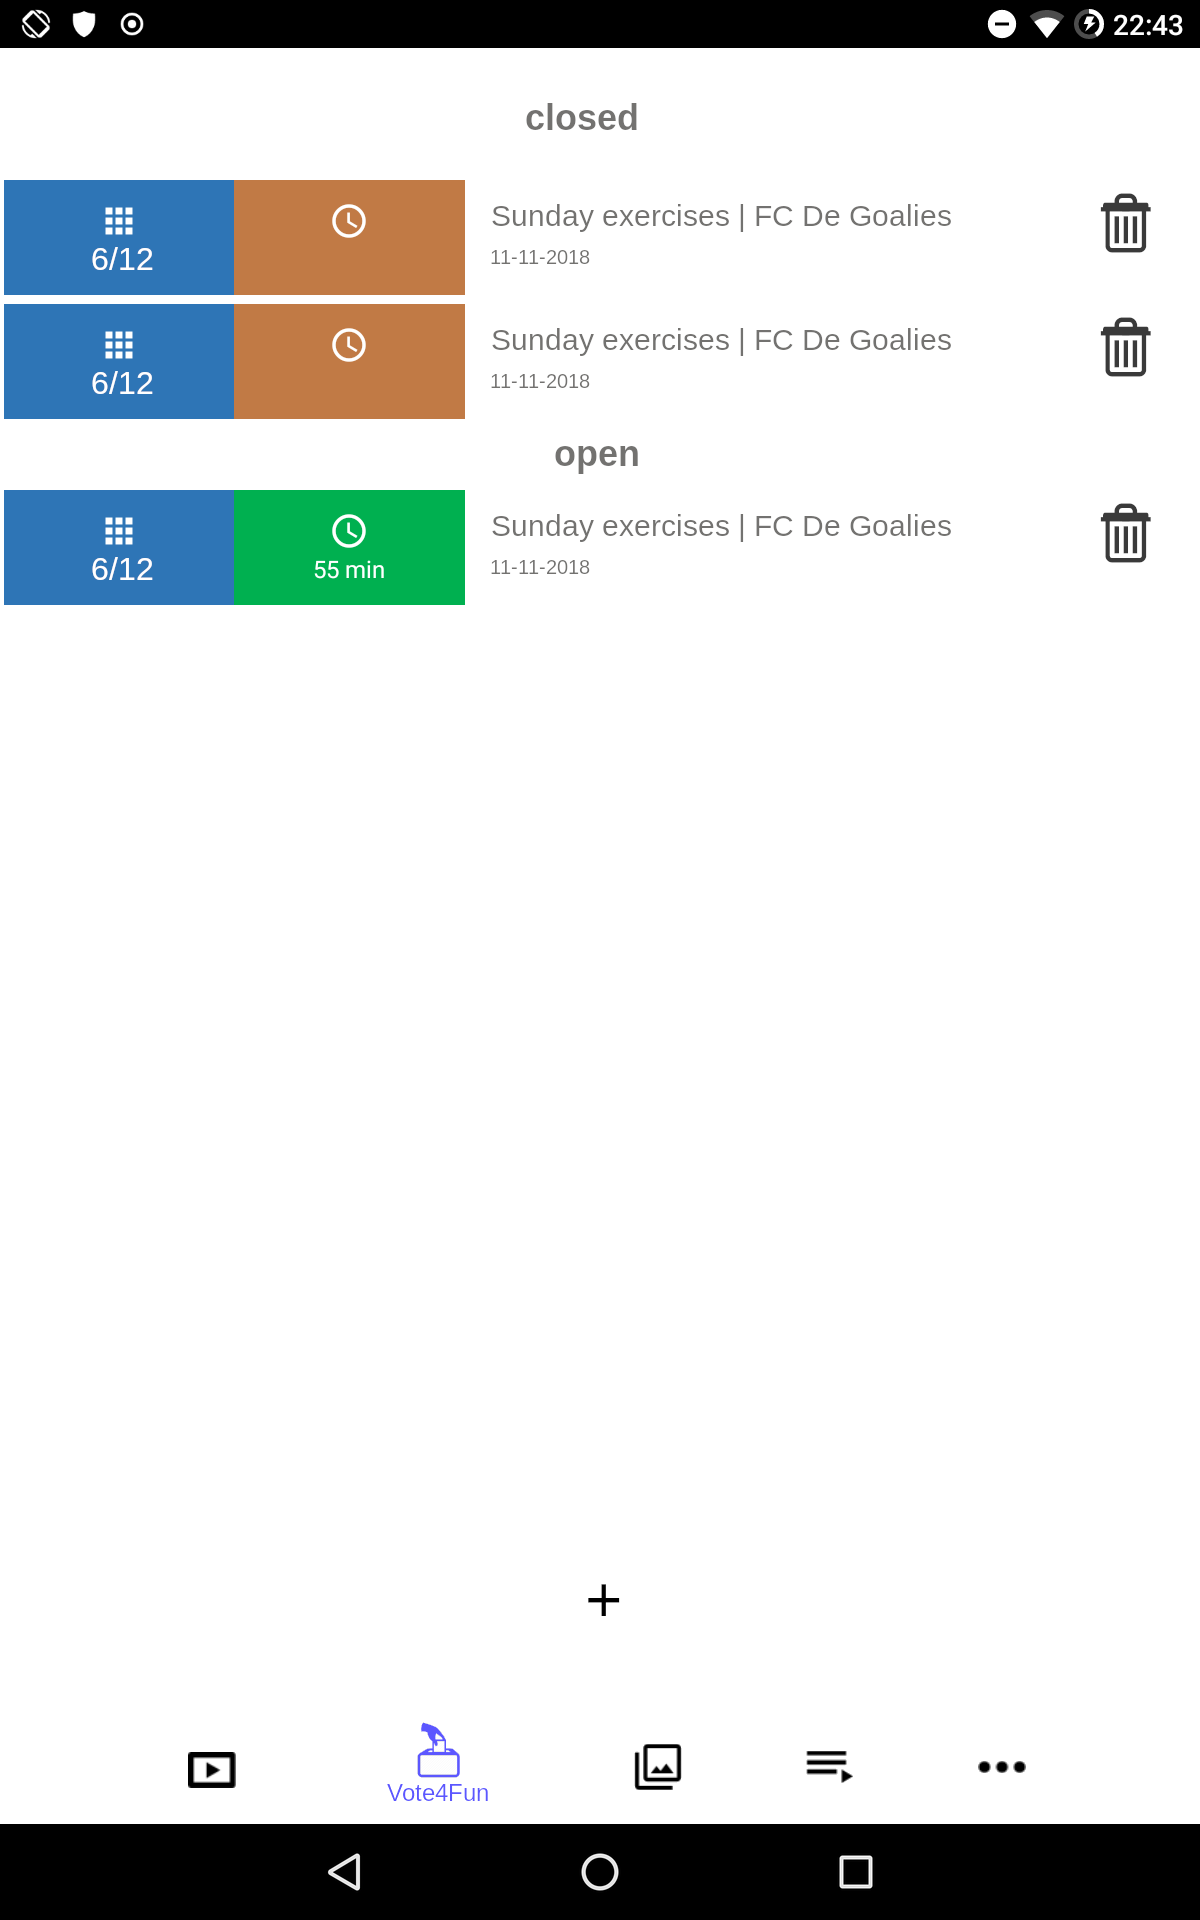
\includegraphics[width=0.4\textwidth]{images/mockups/main-active.png}
        \caption{Mockup Main Overview}
        \label{fig:mockup_main}
    \end{center}
\end{figure}

In Figure \ref{fig:mockup_poll} the mockup shows the overview over a poll. This overview shows how many players voted and how many players vote for each exercise. 
\begin{figure}[H]
    \begin{center}
        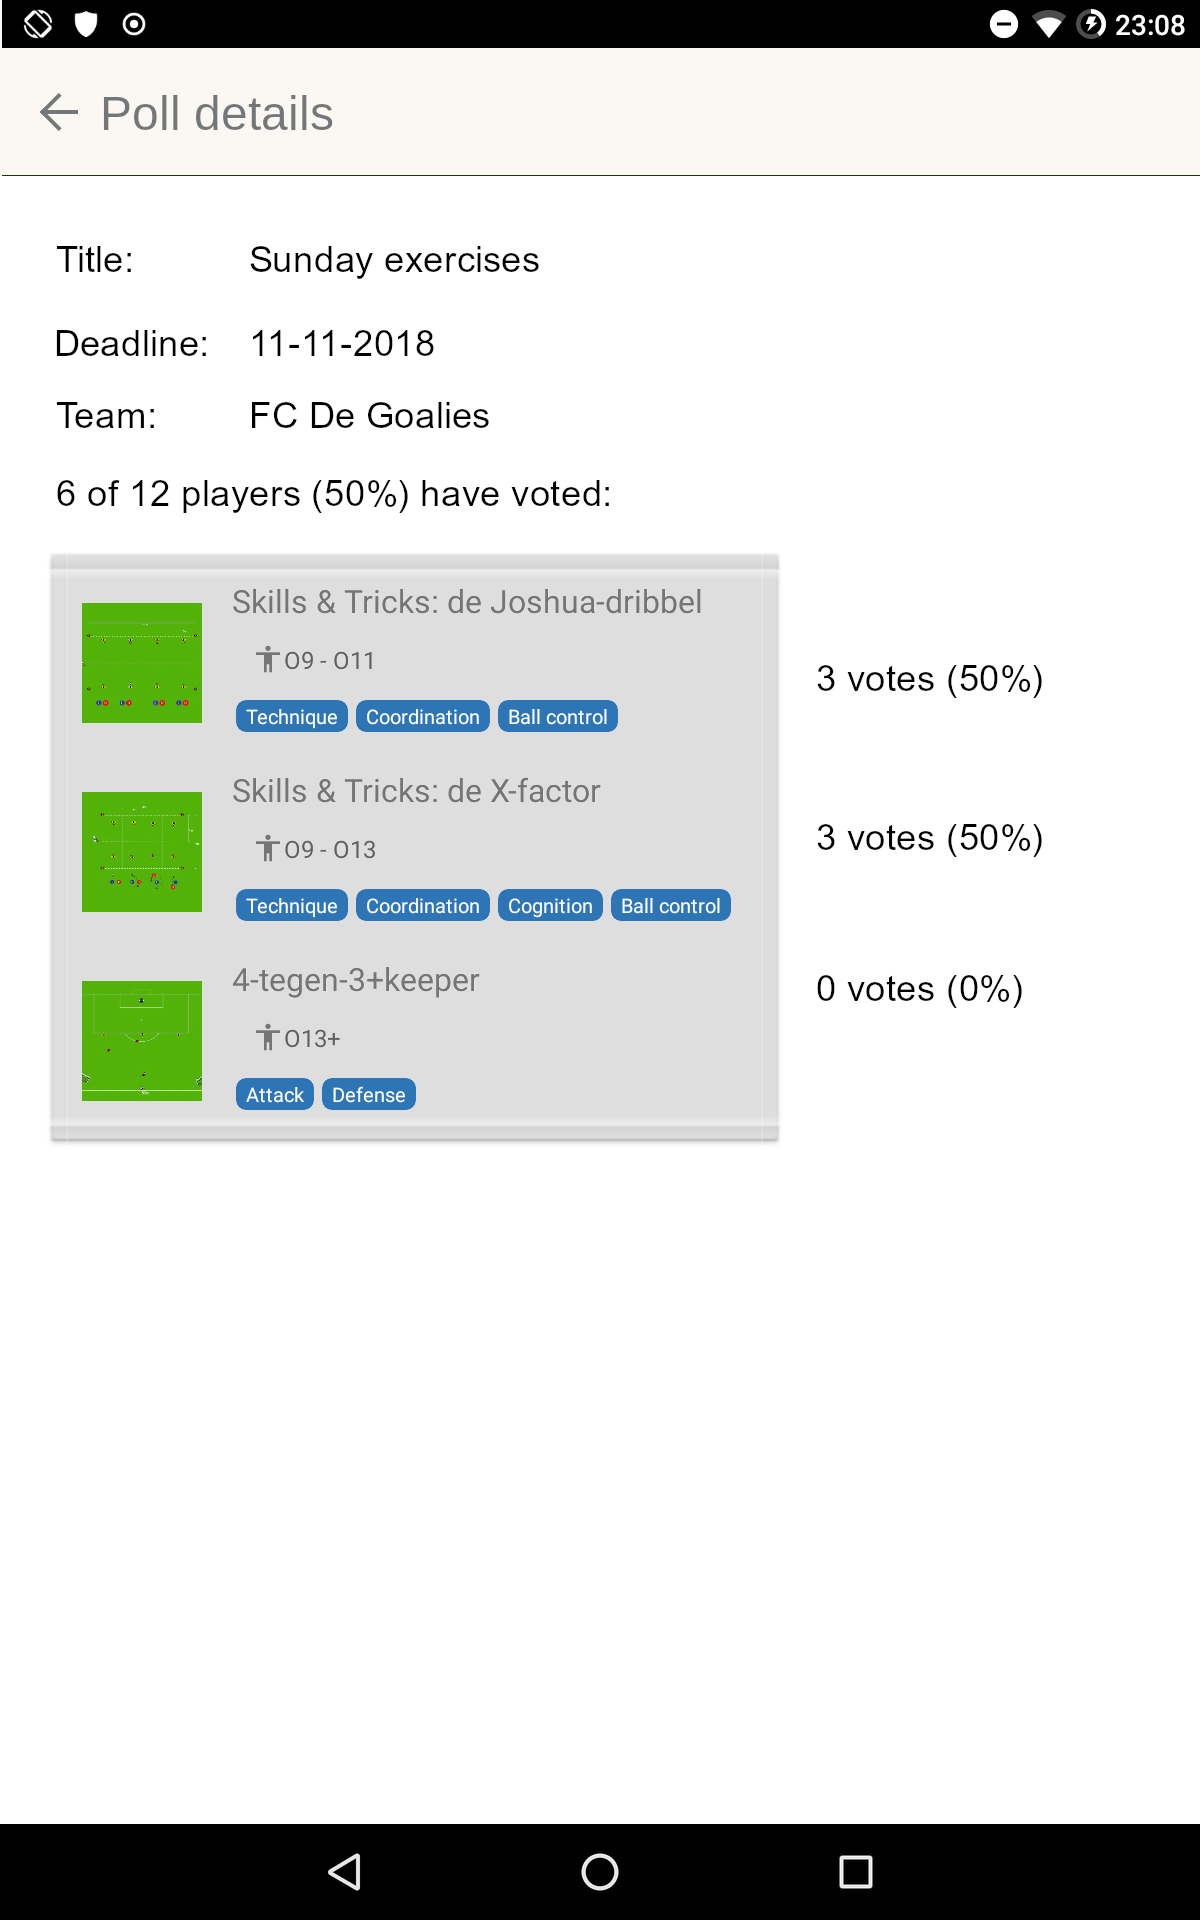
\includegraphics[width=0.4\textwidth]{images/mockups/poll.png}
        \caption{Mockup Poll Dialog}
        \label{fig:mockup_poll}
    \end{center}
\end{figure}

Figure \ref{fig:mockup_select} shows how the coach can selctet the exercise for the poll. The coach is able to select up to 4 and at least 2 exercises. 
\begin{figure}[H]
    \begin{center}
        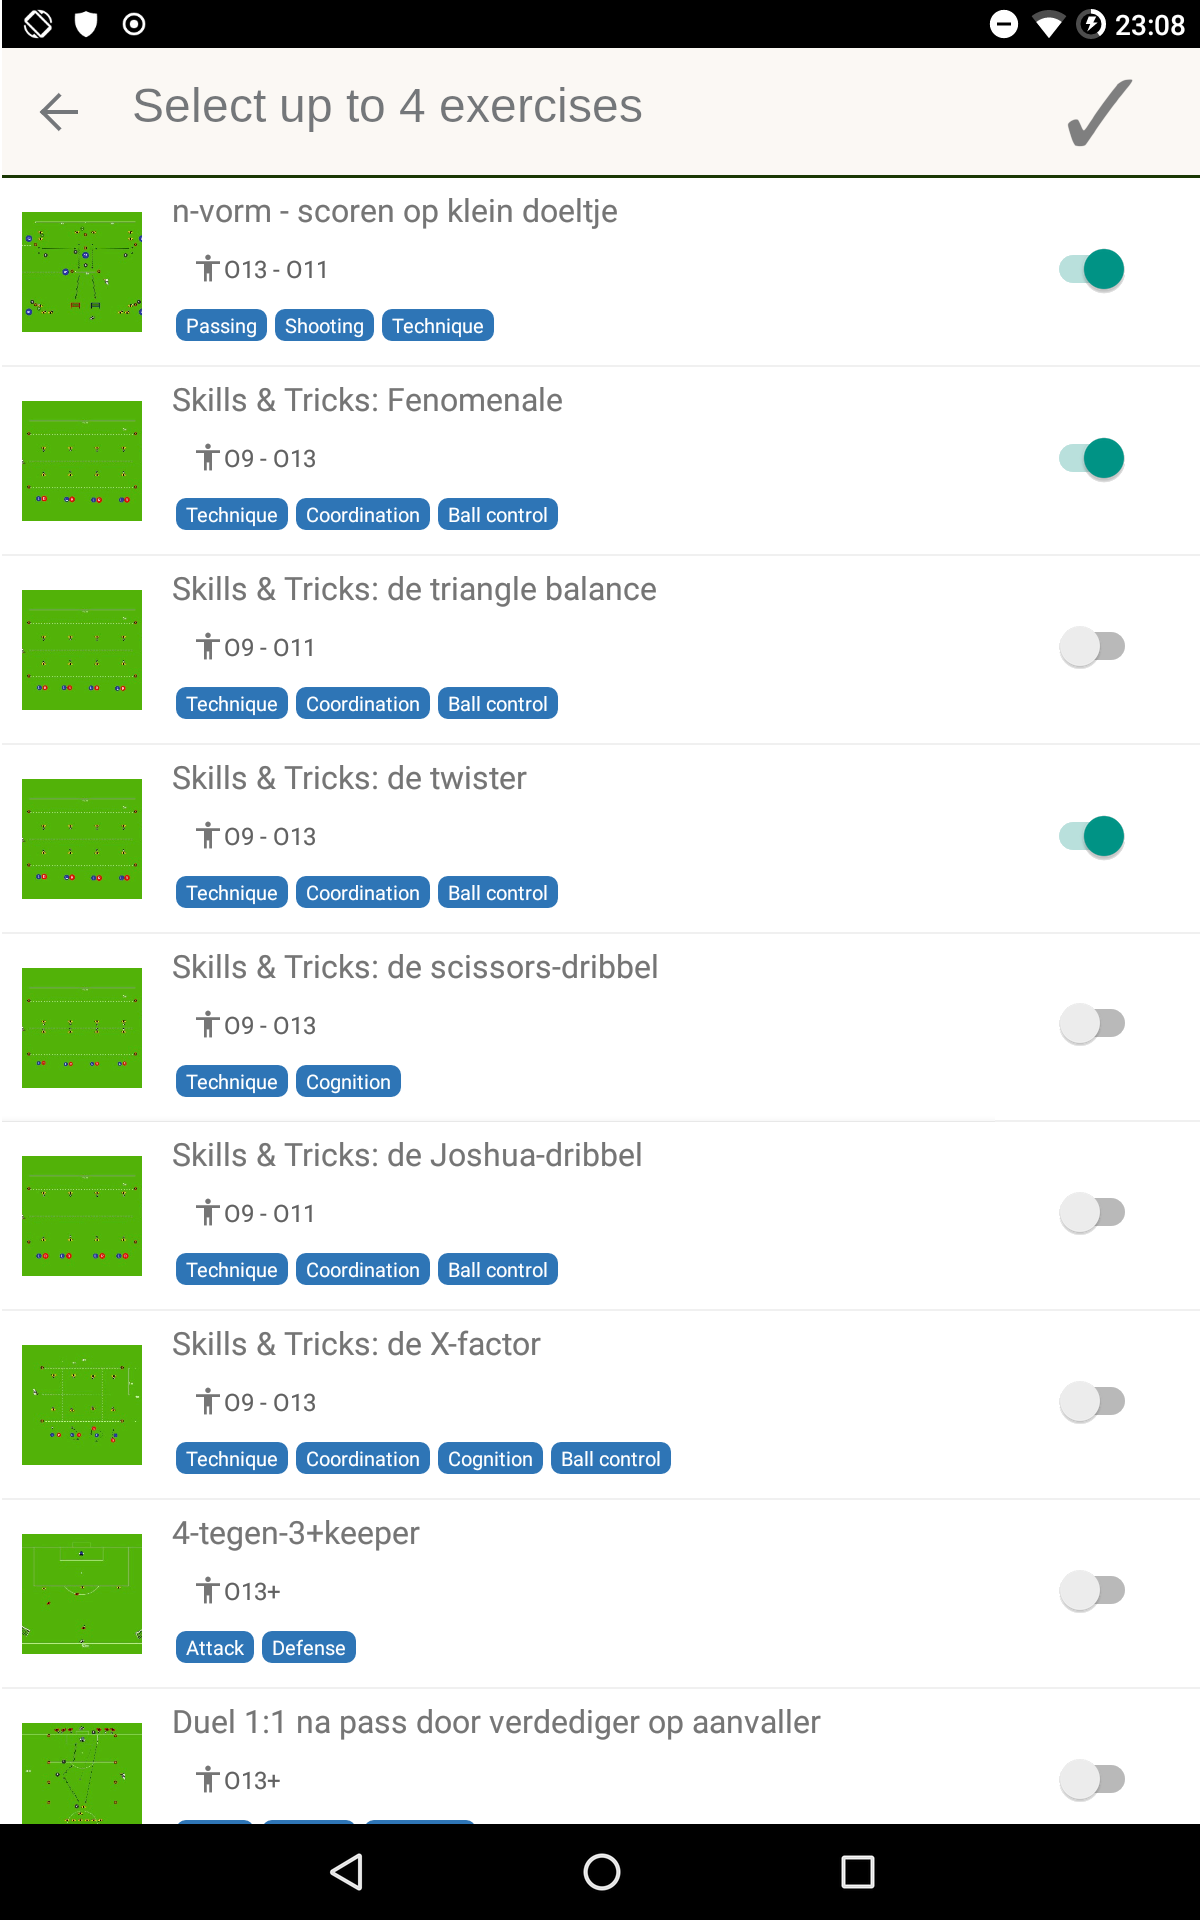
\includegraphics[width=0.4\textwidth]{images/mockups/select-exercises.png}
        \caption{Mockup Select Exercise Dialog}
        \label{fig:mockup_select}
    \end{center}
\end{figure}

\subsection{\textit{Vote4Fun} Object Definition}
\label{ssec:vote4fun_object_definition}

To be able to handle a poll data must be stored, but access to the code was only given to the frontend. Together with the customer we discussed the data we would need and came up with the following representation in \textit{JSON}:

\begin{lstlisting}[language=json,caption=\textit{Vote4Fun} JSON Object,label=lst:vote4fun_json]
{
    id: {
      type: SimpleSchema.RegEx.Id,
      optional: true
    },
    title: {
      type: String,
      min: 1,
      max: 50
    },
    description: {
      type: String,
      max: 10000,
      optional: true
    },
    trainingTarget: {
      type: String,
      max: 200,
      optional: true
    },
    exercises: {
      type: Array
    },
    'exercises.$': {
      type: Object,
      optional: true
    },
    'exercises.$.referenceId': {
      type: String,
      optional: SimpleSchema.RegEx.Id
    },
    'exercises.$.duration': {
      type: Number,
      min: 0,
      max: 30
    },
    'exercises.$.comment': {
      type: String,
      optional: true,
      max: 1000
    },
    'exercises.$.trainingPhase': {
      type: String,
      optional: true,
      max: 50
    },
    fieldSize: {
      type: Number,
      allowedValues: [125, 250, 500, 750, 1000]
    },
    nrOfPlayers: {
      type: Number,
      optional: true,
      min: 0,
      max: 20
    },
    trainingDate: {
      type: String,
      optional: true,
      regEx: /(\d{4}-[01]\d-[0-3]\dT[0-2]\d:[0-5]\d:[0-5]\d\.\d+([+-][0-2]\d:[0-5]\d|Z))|(\d{4}-[01]\d-[0-3]\dT[0-2]\d:[0-5]\d:[0-5]\d([+-][0-2]\d:[0-5]\d|Z))|(\d{4}-[01]\d-[0-3]\dT[0-2]\d:[0-5]\d([+-][0-2]\d:[0-5]\d|Z))/
    },
    teamSharing: {
      type: Object,
      optional: true,
    },
    'teamSharing.teamId': {
      type: String,
      regEx: SimpleSchema.RegEx.id,
    },
    'teamSharing.coach': {
      type: Boolean,
      defaultValue: false,
    },
    'teamSharing.coordinator': {
      type: Boolean,
      defaultValue: false,
    },
    'teamSharing.player': {
      type: Boolean,
      defaultValue: false,
    },
    'teamSharing.vote4fun': {
      type: Boolean,
      defaultValue: false,
    },
    vote4fun: {
      type: Object,
      optional: true,
    },
    'vote4fun.type': {
      type: String,
      allowedValues: ['clubteam', 'open'],
    },
    'vote4fun.title': {
      type: String,
      min: 3,
      max: 40,
    },
    'vote4fun.exercises': {
      type: Array,
      minCount: 2,
      maxCount: 4,
    },
    'vote4fun.exercises.$': {
      type: Object,
    },
    'vote4fun.exercises.$.exerciseId': {
      type: String,
      regEx: SimpleSchema.RegEx.Id,
    },
    'vote4fun.exercises.$.playerIds': {
      type: Array,
    },
    'vote4fun.exercises.$.playerIds.$': {
      type: String,
      regEx: SimpleSchema.RegEx.Id,
    },
    'vote4fun.deadline': {
      type: String,
      regEx: /(\d{4}-[01]\d-[0-3]\dT[0-2]\d:[0-5]\d:[0-5]\d\.\d+([+-][0-2]\d:[0-5]\d|Z))|(\d{4}-[01]\d-[0-3]\dT[0-2]\d:[0-5]\d:[0-5]\d([+-][0-2]\d:[0-5]\d|Z))|(\d{4}-[01]\d-[0-3]\dT[0-2]\d:[0-5]\d([+-][0-2]\d:[0-5]\d|Z))/,
    },
    'vote4fun.guestIDs': {
      type: Array,
      optional: true
    },
    'vote4fun.guestIDs.$': {
      type: String,
      regEx: SimpleSchema.RegEx.Id,
    },
    'vote4fun.showIntermediaResults': {
      type: Boolean,
      defaultValue: false,
    },
    'vote4fun.showFinalResults': {
      type: Boolean,
      defaultValue: false,
    },
    'vote4fun.notificationHoursBeforeDeadline': {
      type: Number,
      defaultValue: 1,
      min: 1,
      max: 24,
    },
    'vote4fun.notificationAfterPercentageVoted': {
      type: Number,
      min: 0,
      max: 100,
    }
}
\end{lstlisting}

The data endpoint was provided by the customer. The idea, besides the self-explaining preference values, is that for every selectable exercise there is an array with user ids. When a user votes for an exercise her or his user id will be saved in that specific array. This way it is always possible to know which user voted for which exercise - and is also open for features like removing a already placed vote.

\subsection{Component Structure}
\label{ssec:component_structure}

Given the component-based structure of the \textit{React Native} framework, some new components had to be designed to implement the necessary functionality of the \textit{Vote4Fun} extension. This section details how the Setup Wizard, which is the main part of the extension, was designed, specifically how it's components are placed in relation to each other and to the existing \textit{Connected.Football} application.

\begin{figure}[H]
    \begin{center}
        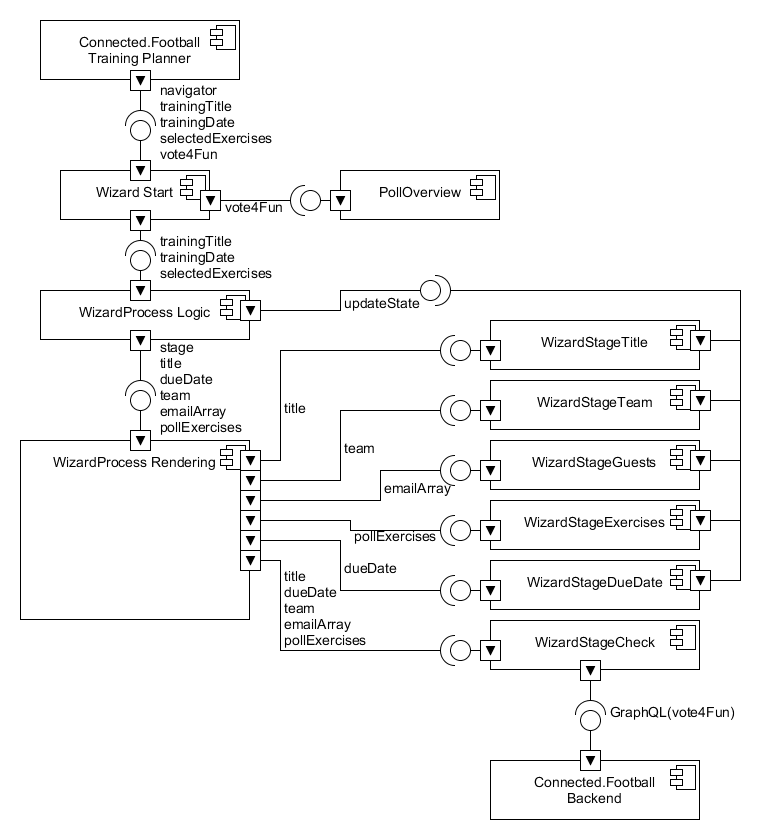
\includegraphics[width=0.9\textwidth]{images/diagrams/component_diagrams/ComponentDiagram_Wizard.png}
        \caption{Component Diagram Poll Setup Wizard}
        \label{fig:component_diagram_wizard}
    \end{center}
\end{figure}

Figure \ref{fig:component_diagram_wizard} shows a component diagram containing all the major components involved in the poll Setup Wizard. The Wizard itself is being used by the \textit{Connected.Football Training Planner}. This was done as a poll is intrinsically linked to a training program and is dependent on one.
\newline
The Wizard itself has an overarching component called \textit{WizardStart}. This is a component that is shown as part of the training planner, displaying either a simple start button to start the setup or an overview in form of the component \textit{PollOverview}, if a \textit{vote4Fun} object is supplied by the training planner. In any case, the component is also supplied with the state of \textit{trainingTitle}, \textit{trainingDate} and \textit{selectedExercises}, as well as a reference to the \textit{navigation} component, since the \textit{WizardProcess} component is called as a new element on the navigation stack of the application.
\newline
The \textit{WizardProcess} is divided into two parts, namely \textit{WizardProcess Logic} and \textit{WizardProcess Rendering}. These are actually parts of the same file, which is a functional component making use of \textit{recompose}. For further information about functional components, see \textit{\ref{ssec:recompose} \nameref{ssec:recompose}}.
\newline
\textit{WizardProcess Logic} handles the business logic and supplies \textit{WizardProcess Rendering} with a state for \textit{stage}, \textit{title}, \textit{dueDate}, \textit{team}, \textit{emailArray} and \textit{pollExercises}. Depending on the value of \textit{stage}, \textit{WizardProcess Rendering} than renders one of the components \textit{WizardStageTitle}, \textit{WizardStageTeam}, \textit{WizardStageGuests}, \textit{WizardStageExercises}, \textit{WizardStageDueDate} and \textit{WizardStageCheck}, in that order.
\newline
Each of the \textit{WizardStage} components is responsible for taking a user's input and sending it to the \textit{WizardProcess Logic} component using a callback function. The \textit{WizardProcess Logic} checks if the user input is valid, which includes the usage of the properties supplied to it by the \textit{WizardStart} component, and sets the state to the user input if it is deemed valid.
\newline
Finally, the \textit{WizardStageCheck} component received all the entered values as properties to render them one last time for the user to check their input. Afterwards, the component triggers a call to the \textit{Connected.Football} backend server, sending a \textit{GraphQL} mutation, which creates a new \textit{Vote4Fun} object on the backend and takes other necessary actions, such as notifying users.
\newline
Aside from the components mentioned above, most components make use of simpler components, such as text entry fields or buttons. These are already supplied by \textit{React Native} or other packages that were loaded. Some custom components were defined over the course of this project, however, they only defined simple logic and rendering and are therefore not mentioned in detail here.